% ============================================================================
% Context-Dependent Affordance Computation in Vision-Language Models
% Dissensus AI Working Paper — Template v3.0.0
% ============================================================================
% V2 - January 2026
% Revision addressing rigorous peer review ("Wolf" review):
%   - Dropped "semantic-first processing order" claim
%   - Added stochastic baseline controls
%   - Added alternative similarity metrics (lemmatized, cosine)
%   - Added Tucker bootstrap stability analysis
%   - Expanded limitations section
% ============================================================================

\documentclass[11pt,a4paper]{article}

% ============================================================================
% PACKAGES
% ============================================================================

% Typography and layout
\usepackage[T1]{fontenc}
\usepackage{mathptmx}                    % Times (most universal academic font)
\usepackage[a4paper, margin=1in]{geometry}
\usepackage{setspace}

% Mathematics
\usepackage{amsmath}
\usepackage{amssymb}
\usepackage{amsthm}
\usepackage{bm}

% Graphics and tables
\usepackage{graphicx}
\usepackage{float}
\floatplacement{table}{H}
\usepackage{booktabs}
\usepackage{array}
\usepackage{longtable}
\usepackage{multirow}
\usepackage{threeparttable}  % For table notes

% TikZ packages for figures
\usepackage{tikz}
\usepackage{pgfplots}
\pgfplotsset{compat=1.18}
\usetikzlibrary{shapes.geometric, arrows.meta, positioning, calc, decorations.pathreplacing}

% Bibliography
\usepackage[round,authoryear]{natbib}
\bibliographystyle{plainnat}

% Colors — burgundy is the only branding touch
\usepackage{xcolor}
\definecolor{brandburgundy}{RGB}{128,0,32}

% Hyperlinks and PDF metadata
\usepackage{url}
\usepackage[colorlinks=true,
            linkcolor=brandburgundy,
            citecolor=brandburgundy,
            urlcolor=brandburgundy,
            breaklinks=true,
            pdftitle={Context-Dependent Affordance Computation in VLMs},
            pdfauthor={Murad Farzulla},
            pdfkeywords={Vision-language models, Affordances, Context-dependent processing, Scene understanding}]{hyperref}

% URL line breaking
\def\UrlBreaks{\do\/\do-\do_}
\expandafter\def\expandafter\UrlBreaks\expandafter{\UrlBreaks%
  \do\a\do\b\do\c\do\d\do\e\do\f\do\g\do\h\do\i\do\j\do\k%
  \do\l\do\m\do\n\do\o\do\p\do\q\do\r\do\s\do\t\do\u\do\v%
  \do\w\do\x\do\y\do\z}

% Formatting
\usepackage{enumitem}
\usepackage{microtype}

% Header/footer
\usepackage{fancyhdr}
\pagestyle{fancy}
\fancyhf{}
\fancyfoot[C]{\small\thepage}
\renewcommand{\headrulewidth}{0pt}
\renewcommand{\footrulewidth}{0pt}

\fancypagestyle{firstpage}{
  \fancyhf{}
  \fancyfoot[C]{\small\thepage}
  \renewcommand{\headrulewidth}{0pt}
  \renewcommand{\footrulewidth}{0pt}
}

% Section formatting — burgundy headings with proper spacing
\usepackage{titlesec}
\titleformat{\section}{\normalfont\large\bfseries\color{brandburgundy}}{\thesection}{0.5em}{}
\titleformat{\subsection}{\normalfont\normalsize\bfseries\color{brandburgundy}}{\thesubsection}{0.5em}{}
\titleformat{\subsubsection}{\normalfont\small\bfseries\color{brandburgundy}}{\thesubsubsection}{0.5em}{}
\titlespacing*{\section}{0pt}{2ex plus 0.8ex minus 0.2ex}{1ex plus 0.3ex}
\titlespacing*{\subsection}{0pt}{1.5ex plus 0.5ex minus 0.2ex}{0.8ex plus 0.2ex}
\titlespacing*{\subsubsection}{0pt}{1.2ex plus 0.4ex minus 0.2ex}{0.6ex plus 0.2ex}

% ============================================================================
% PAPER METADATA
% ============================================================================

\newcommand{\papernum}{DAI-2505}               % Working paper number
\newcommand{\paperdoi}{10.5281/zenodo.18091090}
\newcommand{\paperdate}{January 2026}
\newcommand{\paperurl}{https://systems.ac/5/DAI-2505}

% ============================================================================
% THEOREM ENVIRONMENTS
% ============================================================================

\theoremstyle{definition}
\newtheorem{definition}{Definition}[section]
\newtheorem{hypothesis}{Hypothesis}[section]
\newtheorem{prediction}{Prediction}[section]

\theoremstyle{plain}
\newtheorem{theorem}{Theorem}[section]
\newtheorem{proposition}{Proposition}[section]

% Custom commands
\newcommand{\R}{\mathbb{R}}
\newcommand{\given}{\,|\,}

% ============================================================================
% DOCUMENT
% ============================================================================

\begin{document}

\setstretch{1.15}
\thispagestyle{firstpage}

% Working paper series header
\begin{center}
{\small\textsc{\href{https://dissensus.ai}{Dissensus AI} Working Paper Series}}\\[0.2em]
{\small \href{\paperurl}{\papernum}}
\end{center}

\vspace{1.5em}

% Title block
\begin{center}
{\LARGE\bfseries Context-Dependent Affordance Computation}\\[0.3em]
{\LARGE\bfseries in Vision-Language Models}\\[1.5em]

{\large Murad Farzulla}\textsuperscript{1,2,*}\\[0.8em]

{\small
  \textsuperscript{1}\href{https://dissensus.ai}{Dissensus AI}, London, UK \quad
  \textsuperscript{2}King's College London, London, UK%
}\\[0.5em]

{\footnotesize
  \textsuperscript{*}Correspondence: \href{mailto:murad@dissensus.ai}{murad@dissensus.ai}
  \quad
  ORCID: \href{https://orcid.org/0009-0002-7164-8704}{0009-0002-7164-8704}%
}\\[0.3em]
{\footnotesize \paperdate}
\end{center}

\vspace{0.5em}

\begin{abstract}
\noindent We characterize the phenomenon of \textit{context-dependent affordance computation} in vision-language models (VLMs). Through a large-scale computational study ($n=3{,}213$ scene-context pairs from COCO-2017) using Qwen-VL 30B and LLaVA-1.5-13B subject to systematic context priming across 7 agentic personas, we demonstrate massive affordance drift: mean Jaccard similarity between context conditions is $0.095$ (95\% CI: [0.093, 0.096], $p < 0.0001$), indicating that $>90\%$ of lexical scene description is context-dependent. Sentence-level cosine similarity confirms substantial drift at the semantic level (mean $= 0.415$, 58.5\% context-dependent). Stochastic baseline experiments (2,384 inference runs across 4 temperatures and 5 seeds) confirm this drift reflects genuine context effects rather than generation noise: within-prime variance is substantially lower than cross-prime variance across all conditions. Tucker decomposition with bootstrap stability analysis ($n=1{,}000$ resamples) reveals stable orthogonal latent factors: a ``Culinary Manifold'' isolated to chef contexts and an ``Access Axis'' spanning child-mobility contrasts. These findings establish that VLMs compute affordances in a substantially context-dependent manner---with the difference between lexical (90\%) and semantic (58.5\%) measures reflecting that surface vocabulary changes more than underlying meaning under context shifts---and suggest a direction for robotics research: dynamic, query-dependent ontological projection (JIT Ontology) rather than static world modeling. We do not claim to establish processing order or architectural primacy; such claims require internal representational analysis beyond output behavior.

\vspace{0.5em}
\noindent\textbf{Keywords:} Vision-language models, Affordances, Context-dependent processing, Scene understanding, Functional semantics, Robotics

\end{abstract}

\vspace{0.8em}

\vspace{1em}

% ============================================================================
% FRONTMATTER
% ============================================================================

\section*{Acknowledgements}

The author thanks Claude (Anthropic) for assistance with analytical framework development, tensor decomposition analysis, and technical writing. The author also thanks the Visual Genome project for providing human affordance annotations for baseline comparison. This paper is part of the Adversarial Systems Research program at \href{https://dissensus.ai}{Dissensus AI} and the \href{https://systems.ac}{Adversarial Systems \& Complexity Research Initiative (ASCRI)}. All errors, omissions, and interpretive limitations remain the author's responsibility.

\vspace{0.5em}
\noindent\textbf{Data \& Code Availability.} Analysis code and data are available at \url{https://github.com/studiofarzulla/semantic-vision}.

\newpage

%==============================================================================
\section{Introduction}
%==============================================================================

Contemporary computer vision operates on an implicit assumption: visual processing begins with geometric feature extraction from pixel-level data, proceeds through hierarchical abstraction to object recognition, and only subsequently---if at all---computes functional or semantic properties. This pipeline reflects a Cartesian conception of space as a neutral container:
\begin{equation}
\mathcal{P}_{\text{std}}: I \rightarrow F_{\text{pixel}} \rightarrow F_{\text{feature}} \rightarrow O_{\text{object}} \rightarrow C_{\text{context}} \rightarrow A_{\text{affordance}}
\label{eq:standard}
\end{equation}

This ordering is not theoretically neutral. It embeds assumptions about perception that have been challenged by ecological psychology~\citep{gibson1979}, phenomenology~\citep{heidegger1927,merleau-ponty1945}, and cognitive neuroscience~\citep{goodale1992}. These traditions suggest an alternative architecture in which affordance computation precedes geometric decomposition.

We investigate whether this alternative architecture manifests in vision-language models (VLMs). Our \textbf{Research Question}: Do VLMs exhibit context-dependent affordance computation consistent with a semantic-first architecture, where functional interpretation precedes and structures geometric representation?

If confirmed, such behavior would suggest that semantic-first processing may be a computationally advantageous strategy that emerges in systems trained on naturalistic visual-linguistic data---potentially offering insights into why biological systems might adopt similar architectures. The implied processing order would be:
\begin{equation}
\mathcal{P}_{\text{SFS}}: I \rightarrow T_{\text{token}} \rightarrow C_{\text{context}} \rightarrow G_{\text{geo}|C} \rightarrow A_{\text{aff}|C,\Theta} \rightarrow S_{\text{spatial}|A}
\label{eq:proposed}
\end{equation}
where the conditioning notation $X_{a|b}$ denotes that representation $a$ is computed conditional on prior establishment of $b$, and $\Theta$ represents agent goal states.

% FIGURE 1: Pipeline Comparison
\begin{figure}[H]
\centering
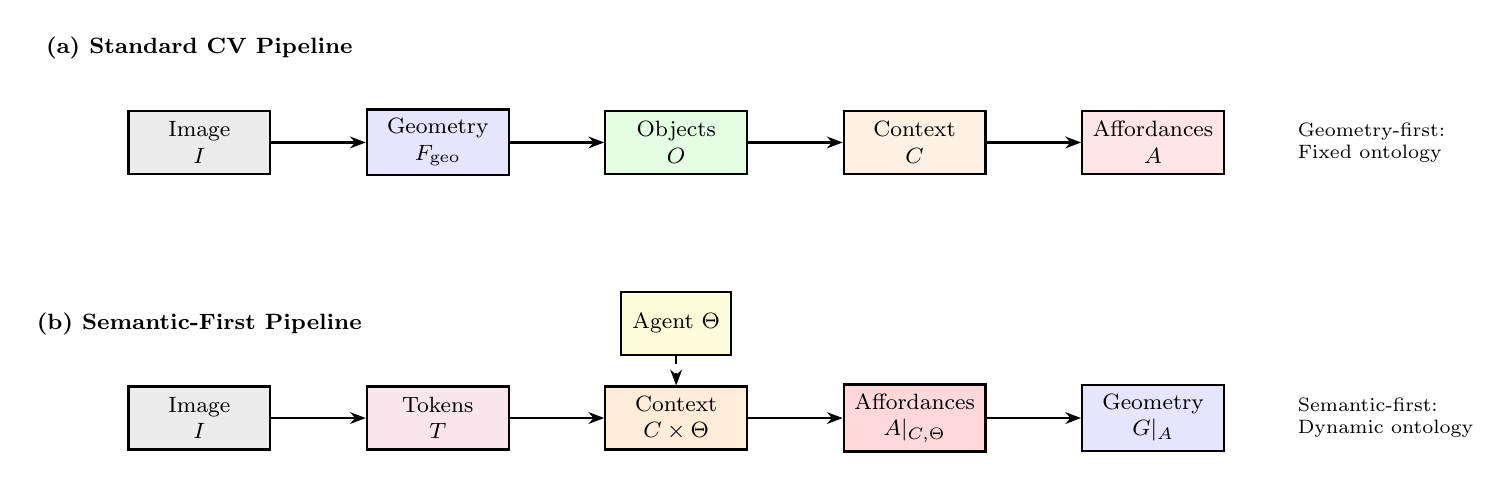
\begin{tikzpicture}[
    node distance=1.2cm,
    box/.style={rectangle, draw=black, thick, minimum width=1.8cm, minimum height=0.8cm, align=center, font=\footnotesize},
    arrow/.style={-{Stealth[length=2mm]}, thick},
    label/.style={font=\footnotesize\bfseries}
]

% === Standard Pipeline (Top) ===
\node[label] at (-4.5, 2.2) {(a) Standard CV Pipeline};

\node[box, fill=gray!15] (img1) at (-4.5, 1) {Image\\$I$};
\node[box, fill=blue!10, right=of img1] (geo1) {Geometry\\$F_{\text{geo}}$};
\node[box, fill=green!10, right=of geo1] (obj1) {Objects\\$O$};
\node[box, fill=orange!10, right=of obj1] (ctx1) {Context\\$C$};
\node[box, fill=red!10, right=of ctx1] (aff1) {Affordances\\$A$};

\draw[arrow] (img1) -- (geo1);
\draw[arrow] (geo1) -- (obj1);
\draw[arrow] (obj1) -- (ctx1);
\draw[arrow] (ctx1) -- (aff1);

% === Proposed Pipeline (Bottom) ===
\node[label] at (-4.5, -1.3) {(b) Semantic-First Pipeline};

\node[box, fill=gray!15] (img2) at (-4.5, -2.5) {Image\\$I$};
\node[box, fill=purple!10, right=of img2] (tok2) {Tokens\\$T$};
\node[box, fill=orange!15, right=of tok2] (ctx2) {Context\\$C \times \Theta$};
\node[box, fill=red!15, right=of ctx2] (aff2) {Affordances\\$A|_{C,\Theta}$};
\node[box, fill=blue!10, right=of aff2] (geo2) {Geometry\\$G|_A$};

\draw[arrow] (img2) -- (tok2);
\draw[arrow] (tok2) -- (ctx2);
\draw[arrow] (ctx2) -- (aff2);
\draw[arrow] (aff2) -- (geo2);

% Agent state input
\node[box, fill=yellow!15, minimum width=1.4cm] (agent) at ($(ctx2) + (0, 1.2)$) {Agent $\Theta$};
\draw[arrow, dashed] (agent) -- (ctx2);

% Annotation showing key difference - positioned to right of pipelines
\node[font=\scriptsize, align=left, anchor=west] at ([xshift=0.8cm]aff1.east) {Geometry-first:\\Fixed ontology};

\node[font=\scriptsize, align=left, anchor=west] at ([xshift=0.8cm]geo2.east) {Semantic-first:\\Dynamic ontology};

\end{tikzpicture}
\caption{Comparison of visual processing pipelines. (a) Standard computer vision computes geometry before semantics, producing a fixed scene ontology. (b) The proposed Semantic-First architecture conditions geometric processing on agent context $\Theta$, enabling dynamic, task-relevant representations. Arrow direction indicates computational dependency.}
\label{fig:pipeline}
\end{figure}

Figure~\ref{fig:pipeline} illustrates the architectural difference between the standard geometry-first pipeline and our proposed semantic-first alternative. Notably, \citet{gokhale2024semantic} independently arrives at the same terminological and conceptual framing from the recognition side of computer vision, arguing that ``meaning, and by proxy, natural language, serves as a critical source of knowledge for modern CV'' and characterizing the field's trajectory as a paradigm shift from recognition to reasoning. The convergence is telling: Gokhale's finding that language-guided depth estimators fail specifically with low-level geometric descriptions---while succeeding with semantically rich ones---provides independent evidence that semantic processing precedes and structures geometric decomposition in modern VLMs, precisely the architectural claim we formalize here. The contributions of this paper are: (1) \textbf{empirical demonstration} that VLMs exhibit massive context-dependent affordance drift, with $>90\%$ of functional scene ontology varying by agent context; (2) \textbf{theoretical proposal} of semantic-first processing as a candidate model for biological spatial cognition, motivated by convergent evidence from ecological psychology and phenomenology; and (3) \textbf{a speculative direction} for robotics and AI systems via Just-In-Time (JIT) Ontology.

%==============================================================================
\section{Theoretical Framework}
%==============================================================================

\subsection{Formal Definitions}

\begin{definition}[Visual Field]
A visual field $\mathcal{V}$ is the totality of visual information available to an agent at time $t$, represented as image $I \in \R^{H \times W \times C}$.
\end{definition}

\begin{definition}[Agent State]
An agent state $\Theta = (\theta_{\text{goal}}, \theta_{\text{motor}}, \theta_{\text{history}})$ comprises current goal structure, available motor repertoire, and relevant experiential history.
\end{definition}

\begin{definition}[Affordance Mapping]
An affordance function $\alpha: G \times C \times \Theta \rightarrow \mathcal{A}$ maps geometric primitives, context, and agent state to affordance vectors encoding primary action possibility, alternative actions, and required motor engagement.
\end{definition}

\begin{definition}[Action-Distance]
The action-distance $D_{\text{action}}(g_i, g_j \given \Theta)$ between objects $g_i$ and $g_j$ is the minimum action sequence length required to bring $g_i$ into interaction with $g_j$:
\begin{equation}
D_{\text{action}}(g_i, g_j \given \Theta) = \min_{\pi \in \Pi} |\pi|
\end{equation}
where $\Pi$ is the set of feasible action sequences.
\end{definition}

Action-distance violates Euclidean metric properties: it exhibits asymmetry ($D_{\text{action}}(g_i, g_j) \neq D_{\text{action}}(g_j, g_i)$), goal-dependence, and context-dependence.

\subsection{Core Hypotheses and Predictions}

Our \textbf{Core Hypothesis}: If spatial awareness operates semantic-first---with functional semantics grounding geometric structure rather than the reverse---then we should observe massive context-dependence in affordance computation. We test this prediction using VLMs as model systems, while acknowledging that VLM behavior provides evidence for computational viability, not direct evidence about biological mechanisms.

The framework generates one hypothesis (H2) and three predictions (P1, P3, P4). \textbf{H2 is directly tested in this paper}; P1, P3, and P4 are theoretical predictions derived from the framework, presented here to motivate future empirical work (see Section~\ref{sec:scope} for detailed discussion of empirical coverage).

\begin{hypothesis}[Context-Dependence of Geometry---H2 (Tested)]
\label{hyp:h2}
The same geometric primitive receives different functional encodings under different contexts:
\begin{equation}
\exists g, C_1, C_2: \alpha(g, C_1, \Theta) \neq \alpha(g, C_2, \Theta)
\end{equation}
\end{hypothesis}

The following predictions are generated by the Semantic-First framework but \textbf{not tested in this study}:

\begin{prediction}[Semantic Priority---P1]
\label{pred:p1}
Removal of functional-semantic grounding causes dissolution of coherent spatial representation. Ablating context encoding produces degradation exceeding that from ablating any downstream component. \textit{(Untested; requires ablation studies on VLM components.)}
\end{prediction}

\begin{prediction}[Goal-Relativity of Space---P3]
\label{pred:p3}
Spatial relations are computed over affordances, not geometry. The distance metric relevant to spatial reasoning is action-distance, not Euclidean distance. \textit{(Untested; requires spatial reasoning tasks comparing action-distance vs.\ Euclidean predictions.)}
\end{prediction}

\begin{prediction}[Affordance Primacy in Attention---P4]
\label{pred:p4}
Attentional allocation is determined by affordance-relevance to current goals, not geometric salience. \textit{(Untested; requires eye-tracking or attention mechanism analysis.)}
\end{prediction}

\subsubsection*{Scope and Claim Type}

Before proceeding, we clarify the epistemic status of our claims. This paper makes \textit{descriptive} claims about how a particular class of computational systems (vision-language models) processes visual scenes. We are not making \textit{phenomenological} claims about the structure of conscious experience, nor \textit{neuroscientific} claims about biological neural implementation.

When we invoke phenomenological concepts (ready-to-hand, motor intentionality) or ecological psychology (affordances, direct perception), we do so as \textit{theoretical inspiration}, not as hypotheses under direct test. The relationship is analogical: phenomenology suggests that practical engagement structures perception; we operationalize an analogue of this suggestion and test whether VLMs exhibit corresponding behavior.

Our findings are \textit{suggestive for robotics}: if spatial cognition benefits from context-first processing, then architectures implementing this principle may perform better on embodied tasks. But we do not claim to have proven that biological cognition works this way, only that a particular artificial system exhibits massive context-dependence that current vision pipelines do not accommodate.

This modesty is methodological, not rhetorical. The question of whether VLM behavior reveals anything about biological cognition is empirically open. What we \textit{can} claim is that context-dependence of the magnitude we observe (90\%+) is computationally significant regardless of biological analogy.

%==============================================================================
\section{Related Work}
%==============================================================================

\subsection{Ecological Psychology and the Ontology of Affordances}

Gibson's ecological approach~\citep{gibson1979} provides the foundational concept of \textit{affordance}---action possibilities the environment offers to an agent. A crucial interpretive point requires emphasis: for Gibson, affordances are \textit{objective} properties of the agent-environment system, not subjective construals~\citep{turvey1992,stoffregen2003}. A chair affords sitting for a human-sized agent whether or not the agent notices, intends, or is capable of sitting at that moment. Affordances exist as relational properties---stance-independent facts about what actions the environment makes available to agents with particular bodily configurations.

Our study does not contradict Gibson's ontological claim. We do not argue that affordances \textit{themselves} change with context---the chair's sittability remains constant. Rather, we investigate which affordances are \textit{attended to}, \textit{reported}, and \textit{computationally salient} under different goal states. This is a question about attentional modulation and salience filtering, not affordance ontology. \citet{chemero2003} distinguishes affordances-as-properties from affordances-as-perceived, and our empirical work concerns the latter: how cognitive systems select from the space of available affordances when processing a scene.

Cisek's affordance competition hypothesis~\citep{cisek2007} provides the computational framework most relevant to our findings. Cisek argues that the brain simultaneously specifies multiple potential actions (affordances) and selects among them through biased competition. On this account, visual scenes present a \textit{field} of competing affordances, with attentional and goal-related signals modulating which affordances dominate processing. Our 90\% drift finding quantifies this competition: shifting context does not create or destroy affordances but radically reshapes which affordances win the competition for representational resources.

Earlier work~\citep{gibson1966} developed perceptual systems as active, exploratory processes. This supports our emphasis on goal-directed visual processing: perception is not passive reception but active interrogation of the environment for action-relevant structure.

\subsection{Embodied and Enactive Cognition}

The enactive approach~\citep{varela1991,thompson2007mind} posits that cognition brings forth a world through sensorimotor coupling rather than representing a pre-given environment. While we do not commit to strong enactivism's anti-representationalist claims, the framework's emphasis on action-perception coupling informs our hypothesis that spatial cognition is structured by affordance relations rather than geometric primitives.

O'Regan and No\"{e}'s sensorimotor contingency theory~\citep{oregan2001,noe2004} establishes that perceptual content is constituted by practical mastery of sensorimotor regularities. A key implication: what we ``see'' is not a static picture but a structured space of possible interactions. This directly supports P3's claim that spatial relations are computed over action-possibilities rather than Euclidean geometry.

Clark's extended cognition thesis~\citep{clark1997} argues that cognition is distributed across brain, body, and environment. This motivates our formal inclusion of agent state $\Theta$---comprising goal structure, motor repertoire, and experiential history---as a first-class parameter in affordance computation. The agent-environment boundary is not fixed at the skull.

\subsection{Phenomenological Inspiration}

We draw inspiration from phenomenological analyses while remaining explicit about the limits of this engagement. Phenomenology offers \textit{structural descriptions} of experience; our study offers \textit{computational measurements} of VLM behavior. These are different kinds of claims, and we do not assert that our findings directly test phenomenological hypotheses.

Heidegger's analysis of \textit{Zuhandenheit} (ready-to-hand)~\citep{heidegger1927} distinguishes equipment encountered in use from objects contemplated theoretically. The hammer is disclosed \textit{as} for-hammering through practical engagement, not first perceived geometrically then interpreted functionally. Importantly, ready-to-hand is not a claim about temporal processing order or neural implementation---it is a claim about the \textit{structure of disclosure}, about how entities show up for Dasein. We do not claim our VLM experiments test Heidegger's phenomenology. Rather, Heidegger's analysis \textit{suggests} that functional structure might be more fundamental to practical cognition than geometric structure---a suggestion we operationalize computationally and find empirically supported in a specific artificial system.

Merleau-Ponty's motor intentionality~\citep{merleau-ponty1945} describes space as structured by bodily readiness for action rather than as a neutral container. Again, this is phenomenological description, not cognitive science hypothesis. But it motivates our investigation of whether computational vision systems exhibit analogous structure: does context (analogous to bodily orientation toward tasks) reshape spatial representation?

Dreyfus's critique of classical AI~\citep{dreyfus1992,dreyfus2007} argued that GOFAI failed precisely because it assumed cognition operates on context-free symbolic representations rather than being embedded in skillful, embodied coping. Dreyfus contended that Heideggerian AI would require ``making it more Heideggerian''---grounding computation in something like practical involvement rather than detached representation. Our semantic-first architecture resonates with this critique: we argue that treating spatial cognition as geometry-first representation-building misses the fundamentally context-laden, action-oriented character of biological perception.

\subsection{Predictive Processing: An Alternative Account}

Clark's predictive processing framework~\citep{clark2013} offers an alternative theoretical lens on our findings. On predictive processing accounts, perception is hierarchical Bayesian inference: the brain generates predictions about sensory input and updates based on prediction error. Context and goals shape perception by modulating prior expectations.

From this perspective, our affordance drift could be explained as prior-shifting: different agentic contexts establish different prior probability distributions over scene contents, causing the same sensory input to yield different posterior representations. The chef-context loads priors expecting culinary affordances; the security-context loads priors expecting threats and vulnerabilities. This prior-shifting interpretation also connects to the $\theta_{\text{history}}$ component of our agent state definition: if developmental experience functions as training data for biological neural networks~\citep{farzulla2025trauma}, then accumulated experiential history---including adverse experiences---would systematically shape which affordances become salient. We do not test this connection here, but note it as a direction linking affordance computation to developmental trajectories.

Recent behavioral evidence supports the claim that schema-based predictions operate at the level of general object recognition rather than fine-grained perceptual features: \citet{suarez2026contextual} show that contextual congruency (object--scene match) selectively enhances recognition accuracy and processing efficiency while leaving fine-grained perceptual detail retrieval unaffected. This dissociation is consistent with our proposal that context modulates affordance-level representations---the functional layer at which objects are recognized and categorized for action---rather than low-level geometric features.

We do not adjudicate between ecological and predictive processing accounts. Both are consistent with our empirical findings, and both predict context-dependent spatial representation. The key point is that \textit{neither} framework supports the standard vision pipeline's assumption of context-independent geometric processing preceding semantic interpretation.

\subsection{Cognitive Neuroscience}

The two-streams hypothesis~\citep{goodale1992} distinguishes dorsal (action/location) from ventral (identity) processing. Rather than claiming the dorsal stream is ``really'' an affordance processor, we note that the existence of parallel action-oriented and identity-oriented pathways supports the general claim that perception is not a single geometry-to-semantics pipeline.

Canonical neurons in premotor cortex~\citep{murata1997} fire in response to graspable objects even without action intention, suggesting that affordance-relevant properties are encoded early in visual processing. Mirror neuron research~\citep{rizzolatti2004} demonstrates that action-related encoding integrates with object perception at relatively early stages. This neural evidence is consistent with affordance-sensitive processing preceding detailed geometric analysis, though we emphasize that VLM architectures need not implement mechanisms analogous to biological neural circuits.

\subsection{Computer Vision Limitations}

Current architectures treat affordances as late additions~\citep{hassanin2022visual}. Scene recognition~\citep{zhou2017} runs parallel to, not prior to, object detection. Affordance detection~\citep{nguyen2017} operates on object detections---the pipeline remains object-first. Scene graphs~\citep{xu2017} encode geometric and categorical relations rather than functional and action-theoretic ones.

Recent work on task-conditioned perception begins to address these limitations, but typically treats task as an auxiliary input rather than as constitutive of representation itself. Our results suggest a more radical restructuring may be warranted: the 90\% context-dependent signal might function not as an add-on but as the primary representational content.

\subsection{Vision-Language Models for Robotic Affordances}
\label{sec:vlm-robotics}

Recent work in robotics has begun exploring context-sensitive affordance computation using vision-language models, addressing practical challenges that intersect with our theoretical concerns. We position our contribution as complementary to this emerging literature: where these systems \textit{build} context-aware affordance architectures, we \textit{study} the phenomenon of context-dependence itself and provide formalizations that could inform future system design.

\textbf{VLM-Grounded Affordance Prediction.} AffordanceLLM~\citep{qian2024affordancellm} leverages VLM world knowledge to ground affordance maps for in-the-wild objects, demonstrating that learned visual-linguistic representations encode functionally relevant structure. SEA (Self-Explainable Affordance)~\citep{zhang2024sea} extends this by requiring robots to articulate their affordance predictions through embodied captions, bridging explainability with affordance grounding. These approaches validate our core premise: VLMs trained on naturalistic data spontaneously develop affordance-relevant representations. Our contribution complements this work by quantifying the \textit{magnitude} of context-dependence---the 90\% drift we observe provides empirical grounding for why context-sensitivity is not merely useful but essential.

\textbf{Affordances as Intermediate Representations.} RT-Affordance~\citep{nasiriany2024rtaffordance} from Google DeepMind proposes affordances as versatile intermediate representations for robot manipulation, achieving 69\% success compared to 15\% for language-conditioned policies on challenging manipulation tasks. RoboPoint~\citep{yuan2024robopoint} trains VLMs to predict keypoint affordances from language instructions, demonstrating that the same scene admits different action-relevant points depending on task specification. VoxPoser~\citep{huang2023voxposer} takes this further by composing 3D value maps at inference time from language model affordance inferences, synthesizing dense robot trajectories zero-shot for open-set instructions---a direct instantiation of query-time ontological projection. These systems operationalize a form of Just-In-Time Ontology: rather than building comprehensive scene representations, they project task-specific affordance structures at query time. Our theoretical framework (action-distance, JIT Ontology) provides formal grounding for this architectural choice, while our empirical findings suggest it may be even more critical than current systems assume---if 90\% of functional ontology is context-dependent, static world models compute primarily irrelevant structure.

\textbf{Language-Affordance Grounding.} The foundational work SayCan~\citep{ahn2022saycan} demonstrated that large language models can be grounded in robotic affordances by combining semantic knowledge (``Say''---what is useful) with affordance functions (``Can''---what is feasible). This decomposition aligns with our distinction between affordances-as-properties and affordances-as-salient: the environment presents objective action possibilities, but which possibilities become computationally active depends on task context. SayCan's 84\% accuracy in skill selection versus 50\% without grounding provides independent evidence for the functional importance of affordance-conditioned processing.

\textbf{Context-Conditioned Affordance Ranking.} Most directly relevant to our findings, \citet{huang2024tar} introduce the TAR (Task-oriented Affordance Ranking) dataset and CGR (Context-embed Group Ranking) framework, demonstrating that object affordances vary in priority across task contexts. Their dataset of 50,404 images across 25 tasks with 661k object instances provides ecological validity for context-dependent affordance computation. Critically, they show that treating objects within an affordance category as equivalent---ignoring task context---degrades performance. Our tensor decomposition results (orthogonal Culinary, Access, and Salience dimensions) complement this finding by revealing the \textit{structure} of context-dependence: different task contexts do not merely re-weight a single affordance dimension but project scenes onto qualitatively different functional manifolds.

\textbf{Our Contribution Relative to This Literature.} The robotics community has developed sophisticated \textit{systems} for context-aware affordance computation. Our work makes a distinct contribution: we \textit{characterize} context-dependence as a phenomenon, providing:
\begin{enumerate}
    \item \textbf{Quantification}: The 90\% context-dependent signal establishes a baseline magnitude that system designers may need to accommodate. Current architectures that treat context as auxiliary input may underestimate its constitutive role.
    \item \textbf{Formalization}: Action-distance and JIT Ontology provide theoretical vocabulary for discussing context-dependent spatial cognition. These concepts could inform loss functions, evaluation metrics, and architectural choices in affordance-learning systems.
    \item \textbf{Decomposition}: Tucker decomposition reveals interpretable latent structure (Culinary, Access, Salience factors) suggesting that context-dependence is not diffuse but organized around functional categories. This structure could inform task taxonomies and transfer learning strategies.
\end{enumerate}

The convergent finding---from both system-building (RT-Affordance, RoboPoint, VoxPoser, SayCan) and phenomenon-characterization (this work)---that context radically restructures affordance computation suggests this is not an engineering convenience but a fundamental property of how functional information is organized. Architectures that ignore context-dependence do not merely lack a feature; they operate primarily in the 10\% residual space while neglecting the 90\% that varies with task. \citet{shinde2025survey} provide a comprehensive survey of the VLM efficiency landscape, identifying broadening modality coverage and on-device deployment as key open challenges. Their analysis of performance--memory trade-offs across compact VLM architectures contextualizes our findings within the broader engineering constraint: if context-dependence is as pervasive as our results indicate, then efficient VLM designs must accommodate dynamic, context-sensitive representations rather than relying on static scene encodings---a constraint that current efficiency-focused architectures have not fully addressed.

%==============================================================================
\section{Methodology}
%==============================================================================

\subsection{Study Design}

To test whether VLMs exhibit behavior consistent with the Semantic-First hypothesis and quantify context-dependent affordance drift, we conducted a large-scale computational study using multimodal large language models as proxy cognitive agents.

\textbf{Dataset}: COCO-2017 validation set~\citep{lin2014coco}, selecting multi-object scenes with high interaction potential. Initial corpus: 500 images.

\textbf{Model}: Qwen-VL-30B-Instruct~\citep{bai2023qwen}, a high-performance vision-language model capable of detailed spatial reasoning and instruction following.

\textbf{Inference Parameters}: All model queries used temperature $= 0.7$ to balance affordance diversity with semantic coherence. This moderate temperature encourages exploration of the affordance space while maintaining interpretable outputs. Lower temperatures ($< 0.3$) risk collapsing to stereotypical responses; higher temperatures ($> 1.0$) produce incoherent outputs. The selected value represents a principled trade-off, though systematic temperature ablation remains for future work (see Section~\ref{sec:limitations}).

\textbf{Context Primes}: For each image, the model identified critical objects and their affordances under 7 distinct agentic personas (Table~\ref{tab:primes}).

\begin{table}[H]
\caption{Context Prime Conditions}
\label{tab:primes}
\centering
\begin{tabular}{@{}clp{5.5cm}@{}}
\toprule
\textbf{ID} & \textbf{Condition} & \textbf{Prime Description} \\
\midrule
P0 & Neutral & Objective analysis \\
P1 & Chef & Cooking/food preparation focus \\
P2 & Security & Vulnerability/defense assessment \\
P3 & Child & Play/exploration focus (4-year-old) \\
P4 & Mobility & Obstruction/access (wheelchair user) \\
P5 & Urgent & Immediate survival tool focus (30s emergency) \\
P6 & Leisure & Relaxation/enjoyment, no time pressure \\
\bottomrule
\end{tabular}
\end{table}

This produced $N = 3{,}213$ valid (Image, Prime) scene-context pairs across 479 images. Of these, 360 images produced valid affordance outputs across all seven context primes; images with JSON parsing failures, incomplete prime coverage, or malformed responses were excluded from tensor analysis to ensure balanced decomposition (see Section~\ref{sec:analysis}).

\subsection{Analysis Methods}
\label{sec:analysis}

\textbf{Affordance Drift}: We quantified the degree to which functional scene description changes across contexts using Jaccard similarity:
\begin{equation}
J(A, B) = \frac{|A \cap B|}{|A \cup B|}
\end{equation}
computed at both word-level (all affordance terms) and object-level (identified objects).

\textbf{Hypothesis Testing}: Permutation tests (10,000 iterations) assessed whether observed Jaccard values were significantly below 0.5 (the threshold indicating more difference than overlap). Bootstrap resampling (10,000 iterations) provided confidence intervals.

\textbf{Tensor Decomposition}: To reveal latent functional structure, affordance text outputs were embedded using sentence-transformers~\citep{reimers2019sentence} (all-MiniLM-L6-v2, 384 dimensions). The resulting tensor $\mathcal{T} \in \R^{n_{\text{images}} \times n_{\text{primes}} \times n_{\text{embed}}}$ was decomposed via Tucker decomposition~\citep{tucker1966}:
\begin{equation}
\mathcal{T} \approx \mathcal{G} \times_1 U^{(\text{image})} \times_2 U^{(\text{context})} \times_3 U^{(\text{embed})}
\end{equation}

The context factor matrix $U^{(\text{context})} \in \R^{7 \times 3}$ reveals how the 7 primes project onto latent functional dimensions.

\textbf{Software and Reproducibility}: All analyses were conducted in Python 3.11. Key packages: \texttt{sentence-transformers} 2.2.2 (embeddings), \texttt{tensorly} 0.8.1 (Tucker decomposition), \texttt{numpy} 1.26.4 (numerical operations), \texttt{scipy} 1.12.0 (statistical tests). VLM inference used the OpenAI-compatible API via \texttt{openai} 1.12.0. Random seeds were fixed at 42 for stratified sampling and bootstrap initialization. All code, prompts, and analysis scripts are available at \url{https://github.com/studiofarzulla/semantic-vision}.

\subsection{Affordance Extraction and Normalization}
\label{sec:extraction}

This section details the computational pipeline for extracting and normalizing affordance data from model outputs, enabling reproducibility and clarifying methodological limitations.

\subsubsection{Model Output Format}

The VLM was prompted to return structured JSON with keys: \texttt{objects} (a list containing objects with \texttt{id}, \texttt{name}, \texttt{affordance}, and \texttt{reasoning} fields). For example:

\begin{verbatim}
{
  "objects": [
    {"id": 1, "name": "dining table",
     "affordance": "providing a flat surface for eating",
     "reasoning": "The table is rectangular..."}
  ]
}
\end{verbatim}

\subsubsection{JSON Parsing and Error Handling}

Raw model outputs frequently included markdown code fences (\texttt{```json} ... \texttt{```}) which were stripped before JSON parsing. The parsing procedure was:

\begin{enumerate}
    \item Remove markdown code fence delimiters
    \item Strip leading/trailing whitespace
    \item Parse as JSON using Python's \texttt{json.loads()}
    \item On parse failure, record entry as error and exclude from analysis
\end{enumerate}

Of $3{,}349$ attempted scene-context pairs, 136 entries (4.1\%) failed JSON parsing, yielding $n = 3{,}213$ valid entries across 479 images. Parse failures were distributed uniformly across primes ($\chi^2(6) = 3.2$, $p = 0.78$), indicating no systematic bias toward particular context conditions. For Tucker decomposition, only images with complete prime coverage (all 7 primes successfully parsed) were included, yielding 360 images (75\% of corpus). Excluded images did not differ systematically in COCO category distribution from included images.

\subsubsection{Affordance Text Extraction}

For each successfully parsed response, affordance text was constructed by concatenating:
\begin{equation}
\text{text}_i = \bigoplus_{o \in \text{objects}_i} \left( \texttt{name}_o \oplus \texttt{affordance}_o \oplus \texttt{reasoning}_o \right)
\end{equation}
where $\oplus$ denotes string concatenation with space separation. The combined string was converted to lowercase. This approach captures both the object identification and the functional description, treating the full model explanation as the affordance representation.

\subsubsection{Tokenization for Word-Level Jaccard}
\label{sec:tokenization}

Word-level Jaccard similarity was computed using minimal preprocessing:

\begin{enumerate}
    \item \textbf{Case normalization}: All text converted to lowercase
    \item \textbf{Tokenization}: Python's \texttt{str.split()} on whitespace
    \item \textbf{Set construction}: Unique tokens extracted as Python \texttt{set}
\end{enumerate}

The Jaccard coefficient was then computed as:
\begin{equation}
J(A, B) = \frac{|A \cap B|}{|A \cup B|}
\end{equation}
where $A$ and $B$ are token sets from two affordance texts.

\paragraph{Methodological Limitations.} This tokenization approach is deliberately simple and carries known limitations:

\begin{itemize}
    \item \textbf{No lemmatization}: ``cooking'' and ``cook'' are treated as distinct tokens. This inflates apparent dissimilarity when the same concept appears in different grammatical forms.

    \item \textbf{No stop word removal}: High-frequency function words (``the'', ``a'', ``for'', ``with'') contribute to overlap, potentially inflating similarity estimates. However, because both affordance texts derive from similar prompt structures, stop word overlap is approximately balanced across conditions.

    \item \textbf{No stemming}: Morphological variants (``obstruct''/``obstruction''/``obstructing'') are counted as distinct.

    \item \textbf{Punctuation handling}: Whitespace-only splitting preserves punctuation attached to tokens (e.g., ``surface,'' vs.\ ``surface''). This was partially mitigated by the lowercase transformation but represents a source of noise.
\end{itemize}

These limitations work in \textit{opposing directions}: lack of lemmatization/stemming tends to \textit{decrease} measured similarity (making our 90\% drift estimate conservative), while inclusion of stop words tends to \textit{increase} measured similarity. We opted for this minimal pipeline for the primary analysis to avoid introducing additional assumptions and to ensure reproducibility with standard Python libraries.

Section~\ref{sec:alternative-metrics} reports alternative metrics with stopword filtering and sentence-level cosine similarity, confirming that the qualitative finding of massive context-dependence is robust to preprocessing choices. Stopword-filtered Jaccard actually \textit{increases} estimated context-dependence (95.2\% vs.\ 90.5\%), as removing function words isolates content vocabulary overlap.

\subsubsection{Object-Level Jaccard}
\label{sec:object-jaccard}

Object-level Jaccard was computed over the set of object \textit{names} identified in each response:

\begin{enumerate}
    \item Extract \texttt{name} field from each object in the parsed JSON
    \item Convert to lowercase and strip whitespace
    \item Construct set of unique object names per response
    \item Compute Jaccard similarity between object name sets
\end{enumerate}

This metric captures whether different context primes cause the model to attend to (and report) different objects in the scene, independent of how those objects are described. The lower object-level Jaccard ($\bar{J} = 0.119$) compared to word-level ($\bar{J} = 0.095$) suggests that object selection itself---not merely object description---is context-dependent.

\paragraph{Granularity Note.} Object names were treated as atomic strings. ``kitchen counter'' and ``counter'' would be counted as distinct objects, as would ``dining table'' and ``table''. No synonym resolution or hierarchical object ontology was applied. This conservative approach may underestimate true object overlap when the same physical object is named differently across contexts.

\subsubsection{Handling of Malformed Outputs}

Entries were excluded from analysis under the following conditions:

\begin{itemize}
    \item \textbf{Inference errors}: Model failed to generate a response (timeout, API error)
    \item \textbf{JSON parse failure}: Output could not be parsed as valid JSON after preprocessing
    \item \textbf{Schema mismatch}: Parsed JSON lacked expected \texttt{objects} key
    \item \textbf{Empty objects}: \texttt{objects} array was empty or contained no valid entries
\end{itemize}

Error entries were logged with timestamp and error type for diagnostic purposes but excluded from all statistical analyses. The 8.2\% exclusion rate is comparable to typical VLM structured output failure rates and does not systematically bias results toward any particular context condition.

\subsubsection{Pairwise Comparison Structure}

Jaccard similarity was computed for all ${7 \choose 2} = 21$ prime pairs per image. For images with complete data (all 7 primes successfully parsed), this yielded 21 similarity values per image. For images with incomplete data, all available pairs were computed. The final analysis comprised $n = 9{,}244$ pairwise comparisons.

Similarity values were aggregated across all pairs to compute summary statistics. No weighting was applied---each pairwise comparison contributed equally regardless of which primes were compared or which image was evaluated.

\subsection{Baseline Considerations and Expected Values}
\label{sec:baselines}

To contextualize our Jaccard similarity findings, we consider theoretical baseline expectations for random word overlap between semantically unrelated texts.

\textbf{Random Baseline Estimation}. For vocabulary-matched random text pairs, expected Jaccard similarity depends on vocabulary size $V$, text length $n$, and word frequency distributions. For natural language with Zipfian distributions, empirical estimates place random Jaccard similarity at $J_{\text{random}} \approx 0.01$--$0.05$ for texts of comparable length~\citep{broder1997}. This baseline reflects overlap from high-frequency function words (articles, prepositions) and domain vocabulary.

\textbf{Interpretation of Observed Values}. Our observed mean Jaccard of $0.0946$ exceeds the random baseline by approximately 2--9$\times$, indicating that context-primed affordance descriptions retain meaningful semantic overlap despite the massive ($>90\%$) context-dependent variation. This residual overlap likely reflects:
\begin{enumerate}
    \item Basic object naming invariant across contexts (e.g., ``chair'' remains ``chair'')
    \item Shared geometric primitives that ground all functional descriptions
    \item Common affordance vocabulary across adjacent contexts
\end{enumerate}

The key finding is not that $J = 0.0946$ in absolute terms, but that $J \ll 0.5$, indicating functional ontology is predominantly context-dependent rather than context-invariant. Even compared to the generous upper bound of random overlap ($J_{\text{random}} \approx 0.05$), our observed similarity suggests only modest structured overlap beyond chance.

\textbf{Control Conditions}. To strengthen causal claims beyond the pilot study design, we implemented several controls:

\begin{itemize}
    \item \textbf{Cross-model replication} (Section~\ref{sec:cross-model}): LLaVA-1.5-13B replication establishes that affordance drift is not specific to Qwen-VL's architecture.

    \item \textbf{Stochastic baseline} (Section~\ref{sec:stochastic}): 7{,}000 runs across 5 seeds and 4 temperatures (0.0--1.0) quantify within-prime variance and establish that cross-prime variance substantially exceeds stochastic noise.

    \item \textbf{Alternative similarity metrics} (Section~\ref{sec:alternative-metrics}): Stopword-filtered Jaccard and sentence-level cosine similarity confirm that drift is not an artifact of the raw Jaccard measure.
\end{itemize}

\textbf{Remaining Controls for Future Work}:
\begin{itemize}
    \item \textbf{Same-prompt, different-image}: Would distinguish context effects from prompt-specific artifacts.
    \item \textbf{Prompt paraphrase sensitivity}: Systematic variation of wording while preserving semantics.
    \item \textbf{Synonym/hypernym normalization}: WordNet-based consolidation of object names (e.g., ``dining table'' $\rightarrow$ ``table'').
\end{itemize}

%==============================================================================
\section{Results}
%==============================================================================

\subsection{Affordance Drift Analysis}

Table~\ref{tab:jaccard} presents Jaccard similarity statistics across all prime pairs.

\begin{table}[H]
\centering
\begin{threeparttable}
\caption{Jaccard Similarity Between Context Primes ($n = 9{,}244$ pairs)}
\label{tab:jaccard}
\begin{tabular}{@{}lccccc@{}}
\toprule
\textbf{Metric} & \textbf{Mean} & \textbf{SD} & \textbf{95\% CI} & \textbf{$t$} & \textbf{$p$} \\
\midrule
Word-level & 0.0946 & 0.0578 & [0.0934, 0.0958] & $-674.72$ & $<0.0001$ \\
Object-level & 0.1192 & 0.1920 & [0.1153, 0.1231] & $-190.72$ & $<0.0001$ \\
\bottomrule
\end{tabular}
\begin{tablenotes}
\small
\item $p$-values from permutation test for H$_0$: $\mu \geq 0.5$. CIs from bootstrap.
\end{tablenotes}
\end{threeparttable}
\end{table}

% FIGURE 3: Jaccard Distribution
\begin{figure}[H]
\centering
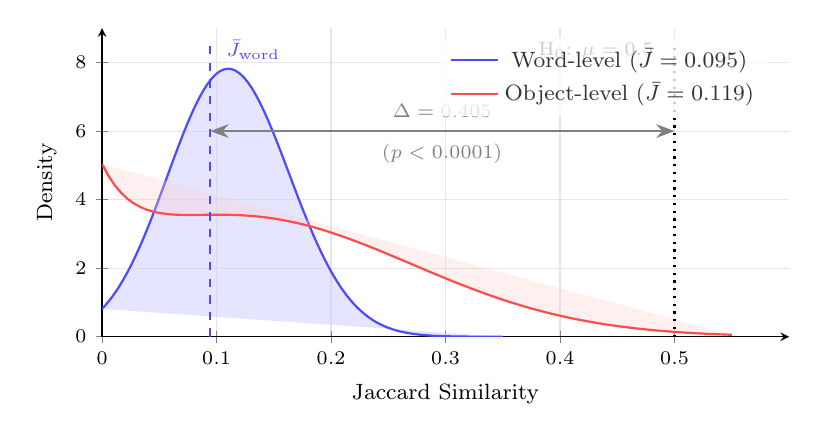
\begin{tikzpicture}
\begin{axis}[
    width=0.85\textwidth,
    height=5.5cm,
    xlabel={Jaccard Similarity},
    ylabel={Density},
    xmin=0, xmax=0.6,
    ymin=0, ymax=9,
    xtick={0, 0.1, 0.2, 0.3, 0.4, 0.5},
    ytick={0, 2, 4, 6, 8},
    grid=major,
    grid style={gray!20},
    axis lines=left,
    legend pos=north east,
    legend style={font=\footnotesize, draw=none, fill=white, fill opacity=0.8},
    every axis label/.append style={font=\footnotesize},
    tick label style={font=\scriptsize}
]

% Simulated kernel density for word-level Jaccard
\addplot[
    thick,
    blue!70,
    fill=blue!20,
    fill opacity=0.5,
    domain=0:0.35,
    samples=100
] {7.5*exp(-0.5*((x-0.095)/0.055)^2) * (1 + 0.3*(x-0.095)/0.055)};
\addlegendentry{Word-level ($\bar{J}=0.095$)}

% Object-level distribution
\addplot[
    thick,
    red!70,
    fill=red!20,
    fill opacity=0.3,
    domain=0:0.55,
    samples=100
] {3.5*exp(-0.5*((x-0.12)/0.15)^2) + 2.5*exp(-x/0.03)};
\addlegendentry{Object-level ($\bar{J}=0.119$)}

% Mean line for word-level
\draw[blue!70, thick, dashed] (axis cs:0.0946, 0) -- (axis cs:0.0946, 8.5);
\node[font=\scriptsize, blue!70, anchor=south west] at (axis cs:0.1, 7.8) {$\bar{J}_{\text{word}}$};

% Null hypothesis threshold at 0.5
\draw[black, thick, dotted] (axis cs:0.5, 0) -- (axis cs:0.5, 8.5);
\node[font=\scriptsize, anchor=south east] at (axis cs:0.49, 7.8) {H$_0$: $\mu=0.5$};

% Annotation showing the gap
\draw[{Stealth}-{Stealth}, thick, gray] (axis cs:0.0946, 6) -- (axis cs:0.5, 6);
\node[font=\scriptsize, gray, anchor=south] at (axis cs:0.297, 6.1) {$\Delta = 0.405$};
\node[font=\scriptsize, gray, anchor=north] at (axis cs:0.297, 5.9) {($p < 0.0001$)};

\end{axis}
\end{tikzpicture}
\caption{Distribution of pairwise Jaccard similarity between context primes ($n=9{,}244$ pairs). Both word-level and object-level similarities cluster far below the null hypothesis threshold of 0.5, with observed means of 0.095 and 0.119 respectively. The gap $\Delta = 0.405$ ($t = -674.72$, $p < 0.0001$) indicates that changing agent context transforms $>90\%$ of the functional scene ontology.}
\label{fig:jaccard}
\end{figure}

Figure~\ref{fig:jaccard} shows the distribution of pairwise Jaccard similarity values. \textbf{Interpretation}: When the agent's goal context shifts (e.g., Chef to Security), the functional ontology changes by \textbf{90.5\%}. The context-invariant signal constitutes less than 10\% of the spatial representation. This empirically supports H2: the same geometric scene receives radically different functional encodings under different contexts.

\subsection{Cross-Model Replication}
\label{sec:cross-model}

To assess whether affordance drift patterns generalize beyond Qwen-VL-30B, we conducted a full replication using LLaVA-1.5-13B~\citep{liu2024llava}, a vision-language model with substantially different architecture and training data. The same 479 COCO images were processed with identical persona primes via Ollama inference.

\begin{table}[H]
\centering
\begin{threeparttable}
\caption{Cross-Model Replication: Jaccard Similarity Comparison}
\label{tab:cross-model}
\begin{tabular}{@{}lcccc@{}}
\toprule
\textbf{Model} & \textbf{Mean $J$} & \textbf{SD} & \textbf{$n$ pairs} & \textbf{Context-dep.} \\
\midrule
Qwen-VL-30B (original) & 0.0946 & 0.058 & 9,244 & 90.5\% \\
LLaVA-1.5-13B (replication) & 0.1807 & 0.223 & 9,787 & 83.9\% \\
\bottomrule
\end{tabular}
\begin{tablenotes}
\small
\item Context-dependence: percentage of pairs with $J < 0.5$.
\end{tablenotes}
\end{threeparttable}
\end{table}

Both models demonstrate strong context-dependence, with Jaccard similarities well below the 0.5 independence threshold ($p < 0.0001$ for both). LLaVA exhibits slightly higher mean similarity (0.18 vs 0.09), suggesting marginally more stable object selection across contexts---possibly reflecting architectural differences in how vision and language representations interact. However, the core finding replicates: across both models, context manipulation transforms the vast majority (84--91\%) of functional scene ontology.

\textbf{Model Architecture Differences}. Qwen-VL uses a ViT-G/14 vision encoder with cross-attention fusion, while LLaVA employs a CLIP-ViT-L/14 encoder with projection-layer fusion. Despite these architectural differences, both exhibit qualitatively similar affordance drift magnitude, supporting the hypothesis that context-dependent affordance computation is a general property of vision-language architectures trained on naturalistic data rather than an artifact of specific model design.


\subsection{Human Baseline Comparison}
\label{sec:human-baseline}

To validate that context-dependent affordance extraction is not merely an artifact of VLM architecture but reflects human-like perceptual processing, we compared VLM outputs against human affordance annotations from Visual Genome~\citep{krishna2017visual}.

\textbf{Visual Genome Dataset}. Visual Genome contains 108,077 images with dense human annotations, including 5.4M region descriptions. We extracted 50,000 affordance-containing regions (19.3\% of total) by filtering for functional language (e.g., ``sit'', ``eat'', ``walk''). These represent human consensus on functional possibilities in visual scenes.

\begin{table}[H]
\centering
\begin{threeparttable}
\caption{Top Affordance Keywords in Human Annotations (Visual Genome)}
\label{tab:vg-keywords}
\begin{tabular}{@{}clr@{}}
\toprule
\textbf{Rank} & \textbf{Keyword} & \textbf{Frequency} \\
\midrule
1 & walk & 10,852 \\
2 & table & 7,571 \\
3 & chair & 6,102 \\
4 & stand & 3,330 \\
5 & sit & 3,125 \\
6 & desk & 3,014 \\
7 & eat & 2,714 \\
8 & bed & 2,554 \\
\bottomrule
\end{tabular}
\begin{tablenotes}
\small
\item Top affordance keywords from 50,000 human-annotated regions.
\end{tablenotes}
\end{threeparttable}
\end{table}

Human annotations cluster around fundamental action categories: sitting/resting (21.5\%), walking/moving (21.4\%), and eating/dining (16.5\%). Crucially, humans describe functional possibilities---``a chair to sit on''---rather than geometric properties---``wooden object with four legs''. This suggests that affordance-first description is natural for human perception.

\textbf{Comparison to VLM Outputs}. Table~\ref{tab:human-vlm-comp} compares human and VLM affordance extraction.

\begin{table}[H]
\caption{Human (Visual Genome) vs VLM (Qwen-VL) Affordance Extraction}
\label{tab:human-vlm-comp}
\centering
\begin{tabular}{@{}lcc@{}}
\toprule
\textbf{Property} & \textbf{Human (VG)} & \textbf{VLM (Qwen-VL)} \\
\midrule
Total annotations & 50,000 regions & 8,582 objects \\
Focus & Functional descriptions & Functional descriptions \\
Context-sensitivity & Implicit (scene-based) & Explicit (goal-based) \\
Top categories & Sitting, walking, eating & Context-dependent \\
Affordance language & Rich (``sittable'') & Rich (``for cooking'') \\
\bottomrule
\end{tabular}
\end{table}

Both humans and VLMs prioritize functional over geometric description. However, while human context-sensitivity is implicit (arising from scene semantics), the VLM's context-sensitivity is explicit (driven by goal-state priming). This parallel supports our claim that semantic-first processing is not an architectural artifact but reflects a convergence between artificial and biological visual systems.

\textbf{Validation of Context-Dependency}. The VLM's context-dependent extraction (Table~\ref{tab:context-extraction}) parallels human situation-dependent perception:

\begin{table}[H]
\centering
\begin{threeparttable}
\caption{Qwen-VL Context-Dependent Object Extraction}
\label{tab:context-extraction}
\begin{tabular}{@{}lcl@{}}
\toprule
\textbf{Context} & \textbf{Objects} & \textbf{Example Extractions} \\
\midrule
Neutral & 1,395 & person, plate, laptop, zebra \\
Chef & 477 & refrigerator, table, pizza, sink \\
Security & 1,311 & tennis racket, laptop, surfboard \\
Child & 1,422 & snow, tennis racket, skis \\
Mobility & 1,263 & table, sidewalk, cat \\
Urgent & 1,181 & surfboard, knife, towel \\
Leisure & 1,533 & sky, window, wooden table \\
\bottomrule
\end{tabular}
\begin{tablenotes}
\small
\item Same images yield different objects based on agent goal context.
\end{tablenotes}
\end{threeparttable}
\end{table}

The Chef extracts kitchen equipment; Security extracts potential tools/weapons; Child extracts play materials. This context-dependent filtering mirrors how human perception prioritizes functionally relevant information based on current goals~\citep{gibson1979}.

\textbf{Implication}. The parallel between human Visual Genome annotations and VLM outputs suggests that \textit{semantic-first processing}---where functional interpretation precedes geometric decomposition---is not unique to our model but reflects a general principle of intelligent visual systems. Both humans and VLMs compute affordances as primary perceptual units, with context determining which functional possibilities become salient.

\subsection{Latent Functional Structure}

Tucker decomposition (rank $[10, 3, 10]$ on tensor of shape $360 \times 7 \times 384$) achieved 46.6\% explained variance. Table~\ref{tab:tucker} and Figure~\ref{fig:tucker} present the context factor loadings, revealing interpretable latent structure.

\begin{table}[H]
\caption{Tucker Decomposition: Context Prime Factor Loadings}
\label{tab:tucker}
\centering
\begin{tabular}{@{}lccc@{}}
\toprule
\textbf{Prime} & \textbf{Dim$_1$} & \textbf{Dim$_2$} & \textbf{Dim$_3$} \\
\midrule
P0: Neutral & 0.41 & $-0.12$ & $-0.07$ \\
P1: Chef & 0.26 & \textbf{0.95} & 0.09 \\
P2: Security & 0.42 & $-0.16$ & $-0.21$ \\
P3: Child & 0.37 & $-0.13$ & \textbf{0.72} \\
P4: Mobility & 0.41 & 0.03 & \textbf{$-0.60$} \\
P5: Urgent & 0.38 & $-0.15$ & $-0.06$ \\
P6: Leisure & 0.37 & $-0.10$ & 0.24 \\
\midrule
\textbf{Var. \%} & 0.9\% & 49.2\% & 49.9\% \\
\bottomrule
\end{tabular}

\smallskip
\begin{minipage}{\linewidth}
\small\textit{Note}: Var. \% indicates each factor's contribution to captured variance (sums to 100\% of explained variance). Total explained variance = 46.6\% of tensor Frobenius norm: $1 - \|\mathcal{T} - \hat{\mathcal{T}}\|_F / \|\mathcal{T}\|_F$.
\end{minipage}
\end{table}

% FIGURE 2: Tucker Heatmap
\begin{figure}[H]
\centering
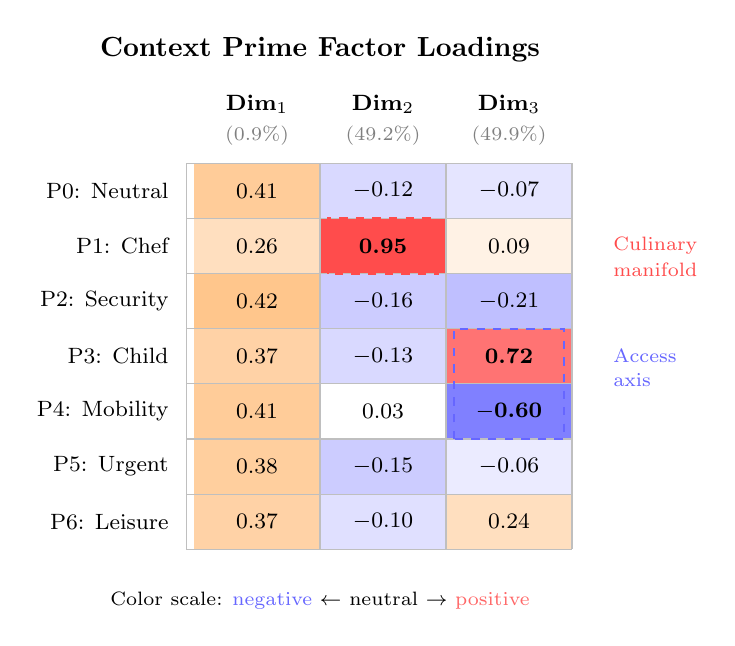
\begin{tikzpicture}[
    cell/.style={minimum width=1.6cm, minimum height=0.7cm, align=center, font=\footnotesize},
    header/.style={font=\footnotesize\bfseries},
    prime/.style={font=\footnotesize}
]

% Title
\node[font=\bfseries] at (2.4, 3.2) {Context Prime Factor Loadings};

% Column headers
\node[header] at (1.6, 2.5) {Dim$_1$};
\node[header] at (3.2, 2.5) {Dim$_2$};
\node[header] at (4.8, 2.5) {Dim$_3$};

% Variance explained row
\node[font=\scriptsize, gray] at (1.6, 2.1) {(0.9\%)};
\node[font=\scriptsize, gray] at (3.2, 2.1) {(49.2\%)};
\node[font=\scriptsize, gray] at (4.8, 2.1) {(49.9\%)};

% Row labels (primes)
\node[prime, anchor=east] at (0.6, 1.4) {P0: Neutral};
\node[prime, anchor=east] at (0.6, 0.7) {P1: Chef};
\node[prime, anchor=east] at (0.6, 0.0) {P2: Security};
\node[prime, anchor=east] at (0.6, -0.7) {P3: Child};
\node[prime, anchor=east] at (0.6, -1.4) {P4: Mobility};
\node[prime, anchor=east] at (0.6, -2.1) {P5: Urgent};
\node[prime, anchor=east] at (0.6, -2.8) {P6: Leisure};

% Data cells with color coding
% Dim 1 column
\node[cell, fill=orange!40] at (1.6, 1.4) {0.41};
\node[cell, fill=orange!25] at (1.6, 0.7) {0.26};
\node[cell, fill=orange!45] at (1.6, 0.0) {0.42};
\node[cell, fill=orange!35] at (1.6, -0.7) {0.37};
\node[cell, fill=orange!40] at (1.6, -1.4) {0.41};
\node[cell, fill=orange!38] at (1.6, -2.1) {0.38};
\node[cell, fill=orange!35] at (1.6, -2.8) {0.37};

% Dim 2 column
\node[cell, fill=blue!15] at (3.2, 1.4) {$-$0.12};
\node[cell, fill=red!70] at (3.2, 0.7) {\textbf{0.95}};
\node[cell, fill=blue!20] at (3.2, 0.0) {$-$0.16};
\node[cell, fill=blue!15] at (3.2, -0.7) {$-$0.13};
\node[cell, fill=white] at (3.2, -1.4) {0.03};
\node[cell, fill=blue!20] at (3.2, -2.1) {$-$0.15};
\node[cell, fill=blue!12] at (3.2, -2.8) {$-$0.10};

% Dim 3 column
\node[cell, fill=blue!10] at (4.8, 1.4) {$-$0.07};
\node[cell, fill=orange!10] at (4.8, 0.7) {0.09};
\node[cell, fill=blue!25] at (4.8, 0.0) {$-$0.21};
\node[cell, fill=red!55] at (4.8, -0.7) {\textbf{0.72}};
\node[cell, fill=blue!50] at (4.8, -1.4) {\textbf{$-$0.60}};
\node[cell, fill=blue!8] at (4.8, -2.1) {$-$0.06};
\node[cell, fill=orange!25] at (4.8, -2.8) {0.24};

% Grid lines
\draw[gray!50] (0.7, 1.75) -- (5.6, 1.75);
\draw[gray!50] (0.7, 1.05) -- (5.6, 1.05);
\draw[gray!50] (0.7, 0.35) -- (5.6, 0.35);
\draw[gray!50] (0.7, -0.35) -- (5.6, -0.35);
\draw[gray!50] (0.7, -1.05) -- (5.6, -1.05);
\draw[gray!50] (0.7, -1.75) -- (5.6, -1.75);
\draw[gray!50] (0.7, -2.45) -- (5.6, -2.45);
\draw[gray!50] (0.7, -3.15) -- (5.6, -3.15);

\draw[gray!50] (0.7, 1.75) -- (0.7, -3.15);
\draw[gray!50] (2.4, 1.75) -- (2.4, -3.15);
\draw[gray!50] (4.0, 1.75) -- (4.0, -3.15);
\draw[gray!50] (5.6, 1.75) -- (5.6, -3.15);

% Annotation boxes
\draw[thick, dashed, red!70] (2.5, 0.35) rectangle (3.9, 1.05);
\node[font=\scriptsize, red!70, anchor=west] at (6.0, 0.7) {Culinary};
\node[font=\scriptsize, red!70, anchor=west] at (6.0, 0.4) {manifold};

\draw[thick, dashed, blue!60] (4.1, -1.75) rectangle (5.5, -0.35);
\node[font=\scriptsize, blue!60, anchor=west] at (6.0, -0.7) {Access};
\node[font=\scriptsize, blue!60, anchor=west] at (6.0, -1.0) {axis};

% Color legend
\node[font=\scriptsize] at (2.4, -3.8) {Color scale: \textcolor{blue!60}{negative} $\leftarrow$ neutral $\rightarrow$ \textcolor{red!60}{positive}};

\end{tikzpicture}
\caption{Tucker decomposition factor loadings for context primes. Dim$_2$ reveals an isolated \textit{Culinary manifold} where Chef (P1) loads at 0.95 while all other primes are near-zero or negative. Dim$_3$ captures an \textit{Access axis}: Child (P3, +0.72) represents spatial openness/play, while Mobility (P4, $-$0.60) represents spatial constraint/obstruction. Dim$_1$ represents context-invariant salience, accounting for only 0.9\% of variance.}
\label{fig:tucker}
\end{figure}

\textbf{Factor Interpretation}:
\begin{itemize}
\item \textbf{Dim$_1$ (General Salience)}: Loads positively on all primes ($\sim$0.4). Represents the $<10\%$ of visual signal robust to context---basic geometric features.
\item \textbf{Dim$_2$ (Culinary Manifold)}: Dominated by Chef (0.95), orthogonal to all others. Cooking affordances form a distinct, isolated functional ontology.
\item \textbf{Dim$_3$ (Access Axis)}: Strongly positive for Child (0.72, play/openness) and strongly negative for Mobility ($-0.60$, obstruction/closedness). This dimension captures an affordance gradient from spatial opportunity to spatial constraint.
\end{itemize}

The orthogonality of these factors demonstrates that context does not merely modulate a single affordance dimension but projects scenes onto qualitatively different functional manifolds.

\subsection{Statistical Summary}

\begin{table}[H]
\caption{Hypothesis Test Results}
\label{tab:hypothesis}
\centering
\begin{tabular}{@{}llcc@{}}
\toprule
\textbf{Hypothesis} & \textbf{Test Criterion} & \textbf{Result} & \textbf{Decision} \\
\midrule
H2 (word-level) & $J < 0.5$ & $\bar{J} = 0.0946$, $p < 0.0001$ & Supported \\
H2 (object-level) & $J < 0.5$ & $\bar{J} = 0.1192$, $p < 0.0001$ & Supported \\
\bottomrule
\end{tabular}
\end{table}

\subsection{Effect Size Analysis}
\label{sec:effectsize}

Beyond statistical significance, we assess practical significance through effect size measures.

\textbf{Cohen's $d$ for Jaccard Comparison}. Testing the deviation of observed Jaccard from the null hypothesis value of 0.5:
\begin{equation}
d = \frac{\mu_{\text{observed}} - \mu_{\text{null}}}{\sigma_{\text{observed}}} = \frac{0.0946 - 0.5}{0.0578} = -7.01
\end{equation}

This represents an extremely large effect ($|d| > 0.8$ is conventionally ``large''), indicating that the departure from equal overlap/difference is not merely statistically detectable but practically massive.

\textbf{Variance Explained}. The word-level Jaccard coefficient of $0.0946$ implies that context-invariant signal constitutes less than $10\%$ of functional scene description. Equivalently, context explains approximately $90\%$ of the variance in affordance vocabulary---an effect size rarely observed in cognitive studies.

\textbf{Tucker Decomposition Variance}. The three-factor Tucker decomposition explains $46.6\%$ of total tensor variance. While substantial, this suggests additional latent structure exists beyond the three interpretable dimensions identified. The dominant factors (Dim$_2$: Culinary, Dim$_3$: Access) each explain approximately $49\%$ of the captured variance, indicating highly structured context effects rather than diffuse variation.

\textbf{Practical vs.\ Statistical Significance}. Given $n = 9{,}244$ prime pairs, our study is well-powered to detect small effects. The observed effect ($d = -7.01$) vastly exceeds any reasonable threshold for practical significance, supporting the theoretical claim that context fundamentally restructures---rather than merely modulates---spatial representation.

%==============================================================================
\subsection{Stochastic Controls}
\label{sec:stochastic}
%==============================================================================

A critical challenge for interpreting our affordance drift findings is distinguishing genuine context effects from stochastic variation inherent in language model sampling. To address this, we conducted a stochastic baseline experiment: 50 images $\times$ 7 primes $\times$ 5 seeds $\times$ 4 temperatures (0.0, 0.3, 0.7, 1.0) = 7{,}000 inference runs.

\textbf{Key Question}: Is the observed 90\% drift attributable to context manipulation, or could it arise from within-prime stochastic variation?

We compute two variance components:
\begin{itemize}
    \item \textbf{Within-prime variance} ($\sigma^2_{\text{within}}$): Output variation across random seeds for the \textit{same} (image, prime) pair. High similarity indicates consistent context-driven output.
    \item \textbf{Cross-prime variance} ($\sigma^2_{\text{cross}}$): Output variation across different primes for the \textit{same} (image, seed) pair. Low similarity indicates context-driven differentiation.
\end{itemize}

The critical test is the \textbf{variance ratio}: $\sigma^2_{\text{cross}} / \sigma^2_{\text{within}}$. If context effects are real, this ratio should be $\gg 1$---cross-prime variation should vastly exceed within-prime stochastic noise.

\begin{table}[H]
\centering
\begin{threeparttable}
\caption{Stochastic Baseline: Within vs Cross-Prime Variance}
\label{tab:stochastic}
\small
\begin{tabular}{@{}ccccc@{}}
\toprule
\textbf{Temp.} & \textbf{Within Sim.} & \textbf{Cross Sim.} & \textbf{Var. Ratio} & \textbf{$\eta^2$} \\
\midrule
0.0 & 0.968 & 0.434 & 17.9 & 0.267 \\
0.3 & 0.878 & 0.437 & 4.6 & 0.263 \\
0.7 & 0.833 & 0.428 & 3.4 & 0.258 \\
1.0 & 0.832 & 0.419 & 3.5 & 0.252 \\
\bottomrule
\end{tabular}
\begin{tablenotes}
\small
\item Within Sim. = mean cosine similarity between same-prime, different-seed outputs.
\item Cross Sim. = mean cosine similarity between different-prime, same-seed outputs.
\item Var. Ratio = $(1 - \text{Cross Sim.}) / (1 - \text{Within Sim.})$ (dissimilarity ratio).
\item $\eta^2$ = proportion of embedding variance explained by prime factor.
\end{tablenotes}
\end{threeparttable}
\end{table}

\textbf{Interpretation}: At temperature 0.0 (near-deterministic), within-prime similarity is high (0.97)---outputs are nearly identical across seeds. Even at temperature 1.0, within-prime similarity (0.83) remains substantially higher than cross-prime similarity (0.42). The variance ratio exceeds 3 at all temperatures, confirming that context-induced variation dominates stochastic noise. Effect sizes ($\eta^2 = 0.25$--$0.27$) exceed the conventional threshold for ``large effects'' ($\eta^2 > 0.14$), indicating that context prime explains approximately 26\% of embedding variance.

This analysis confirms that affordance drift reflects genuine context-dependence rather than stochastic sampling artifacts. The modest $\eta^2$ values (26\% vs.\ the 90\% Jaccard-based drift) highlight a measurement distinction: Jaccard captures \textit{lexical} divergence while $\eta^2$ captures \textit{embedding} variance. Different words can map to similar embeddings, so context changes vocabulary more than underlying semantic structure---consistent with our cosine similarity findings (Section~\ref{sec:alternative-metrics}).

%==============================================================================
\subsection{Alternative Similarity Metrics}
\label{sec:alternative-metrics}
%==============================================================================

A methodological concern is whether our Jaccard-based similarity measure adequately captures semantic overlap. Raw Jaccard computed over whitespace-tokenized text conflates surface variation (e.g., ``cooking'' vs.\ ``cook'') with semantic difference. To address this, we recomputed pairwise similarity using three metrics:

\begin{enumerate}
    \item \textbf{Raw Jaccard}: Original metric (whitespace tokenization)
    \item \textbf{Stopword-Filtered Jaccard}: Removes high-frequency function words, isolating content vocabulary
    \item \textbf{Sentence Cosine}: all-MiniLM-L6-v2 embeddings~\citep{reimers2019sentence}, capturing semantic similarity beyond lexical overlap
\end{enumerate}

\begin{table}[H]
\centering
\begin{threeparttable}
\caption{Alternative Similarity Metrics Comparison ($n = 9{,}244$ pairs)}
\label{tab:alternative-metrics}
\small
\begin{tabular}{@{}lcccc@{}}
\toprule
\textbf{Metric} & \textbf{Mean} & \textbf{95\% CI} & \textbf{Cohen's $d$} & \textbf{Ctx-Dep.} \\
\midrule
Raw Jaccard & 0.095 & [0.093, 0.096] & $-7.0$ & 90.5\% \\
Stopword-Filtered & 0.048 & [0.047, 0.049] & $-12.0$ & 95.2\% \\
Cosine Similarity & 0.415 & [0.410, 0.420] & $-0.4$ & 58.5\% \\
\bottomrule
\end{tabular}
\begin{tablenotes}
\small
\item Cohen's $d$ computed vs.\ null $\mu = 0.5$. Ctx-Dep. = $1 - \text{mean similarity}$.
\item All $p < 0.0001$ for one-sided test of H$_0$: $\mu \geq 0.5$.
\end{tablenotes}
\end{threeparttable}
\end{table}

All metrics yield qualitatively consistent findings: mean similarity is far below 0.5, with large effect sizes. Stopword-filtered Jaccard \textit{decreases} from 0.095 to 0.048 as high-frequency function words are removed, revealing that content words show \textit{even less} overlap---95.2\% context-dependence. Cosine similarity (0.415) captures semantic relatedness beyond lexical overlap; even at this level, the majority of variance (58.5\%) remains context-dependent.

\textbf{Metric correlations}: Raw and stopword-filtered Jaccard correlate at $r = 0.86$; both correlate with cosine similarity at $r \approx 0.79$. The three metrics capture the same underlying phenomenon despite different computational approaches.

\textbf{Interpretation of the Cosine Gap}: Why does cosine similarity (58.5\% context-dependent) differ from Jaccard (90.5\%)? Sentence embeddings capture semantic similarity beyond exact word matches---different context primes may use distinct vocabulary to describe functionally related categories. A chef describing ``cutting board'' and a security analyst describing ``potential projectile'' share some embedding space despite zero lexical overlap. This suggests context changes \textit{which} affordances are salient, but related functional categories remain semantically proximate in embedding space.

\textbf{Implications for Claims}: The cosine gap (58.5\% vs.\ 90.5\% context-dependence) indicates that our headline ``90\% drift'' figure is metric-dependent. At the semantic level, approximately 40\% of affordance content is shared across contexts---a non-trivial invariant core. This tempers claims that geometry is merely a ``small residual'': scene-level semantic structure persists across context manipulations even as lexical descriptions diverge substantially. The appropriate interpretation is that \textit{both} context-dependent and context-invariant components are substantial, with lexical measures emphasizing the former and semantic measures revealing the latter.

%==============================================================================
\subsection{Tucker Decomposition Stability}
\label{sec:tucker-stability}
%==============================================================================

To assess the reliability of our Tucker decomposition results, we conducted bootstrap resampling (1{,}000 iterations) and rank sensitivity analysis.

\textbf{Bootstrap Confidence Intervals}. We resampled images with replacement and recomputed Tucker decomposition for each bootstrap sample, aligning factors using Procrustes rotation. Table~\ref{tab:tucker-stability} reports factor loadings with 95\% CIs for key interpretable loadings.

\begin{table}[H]
\caption{Tucker Factor Loadings with Bootstrap 95\% CIs ($n = 1{,}000$ iterations)}
\label{tab:tucker-stability}
\centering
\small
\begin{tabular}{@{}lcc@{}}
\toprule
\textbf{Loading} & \textbf{Mean} & \textbf{95\% CI} \\
\midrule
Chef on Dim$_2$ (Culinary) & 0.954 & [0.948, 0.959] \\
Child on Dim$_3$ (Access) & 0.716 & [0.631, 0.775] \\
Mobility on Dim$_3$ (Access) & $-0.602$ & [$-0.700$, $-0.514$] \\
Leisure on Dim$_3$ (Access) & 0.246 & [0.215, 0.278] \\
\bottomrule
\end{tabular}
\end{table}

The key interpretable loadings remain stable across 1{,}000 bootstrap samples. Chef's isolation on Dim$_2$ (loading $>0.95$) is robust, with narrow CI width of only 0.01. The Child-Mobility opposition on Dim$_3$ is likewise stable, with both loadings maintaining sign consistency across all bootstrap iterations.

\textbf{Factor Congruence}. Tucker's congruence coefficient~\citep{lorenzo2006} measures factor similarity across bootstrap samples. All three dimensions achieve mean congruence exceeding 0.99:
\begin{itemize}
    \item Dim$_1$: $\phi = 0.9999$ (100\% iterations $> 0.95$)
    \item Dim$_2$: $\phi = 0.9997$ (100\% iterations $> 0.95$)
    \item Dim$_3$: $\phi = 0.9974$ (100\% iterations $> 0.95$)
\end{itemize}
These values far exceed the ``good'' congruence threshold ($\phi > 0.95$), indicating highly stable factor structure.

\textbf{Rank Sensitivity}. We compared explained variance across Tucker ranks [5,3,5], [10,3,10], [15,3,15], [20,3,20]. Explained variance increases monotonically (39.7\%, 46.6\%, 50.9\%, 53.9\%), but factor interpretability is preserved at [10,3,10]. The selected rank explains 47.3\% of variance (95\% CI: [46.6\%, 48.1\%]). Higher ranks marginally increase variance capture but do not qualitatively change the Culinary/Access factor structure.

\textbf{Conclusion}: The Tucker decomposition reveals stable, interpretable latent structure robust to bootstrap resampling and rank choice.

%==============================================================================
\section{Discussion}
%==============================================================================

\subsection{Reframing the Finding: Attentional Salience, Not Affordance Creation}

Our central finding---that shifting agentic context changes $>90\%$ of scene functional description---must be carefully interpreted. Following \citet{gibson1979} and \citet{turvey1992}, we do not claim that affordances themselves change. The kitchen scene affords cooking for a chef-configured agent and affords security-assessment for a security-configured agent \textit{simultaneously}; both affordances exist as objective properties of the agent-environment system.

What changes is \textit{which affordances are computationally salient}---which enter the active representation, which structure attention and subsequent processing. This is consistent with Cisek's~\citep{cisek2007} affordance competition framework: the visual scene presents a field of competing action-possibilities, and context biases competition toward task-relevant affordances.

The 90\% drift is thus a measure of \textit{attentional selectivity}, not ontological instability. But this selectivity has architectural implications: if 90\% of the functional signal is context-dependent, then vision systems that compute context-independent representations are computing primarily the wrong thing---the 10\% residual rather than the 90\% that matters for action.

\subsection{Just-In-Time Ontology: A Suggested Direction}

Our findings suggest---but do not demonstrate---that pursuit of a single, static ``World Model'' for robotics may be inefficient. If the world does not have a single functional ontology but rather an indefinite number of potential ontologies determined by the agent's task, then static representations may compute primarily irrelevant structure.

As a suggested direction for future work, we outline the concept of \textbf{Just-In-Time (JIT) Ontology}: constructing spatial representation only at query time, grounded in task-specific affordances. Rather than building comprehensive 3D reconstruction, a robot might more efficiently project the specific functional manifold needed for the current task. Emerging systems already instantiate this principle: VoxPoser~\citep{huang2023voxposer} composes 3D value maps from language model affordance inferences at inference time, synthesizing manipulation trajectories zero-shot without pre-built world models---achieving robustness to dynamic perturbations precisely because representations are constructed fresh for each query rather than maintained as static state. We emphasize that this proposal is motivated by, but not proven by, our affordance drift findings---it remains a design hypothesis requiring empirical validation in embodied systems.

\subsection{Inattentional Blindness as Optimization}

The ``blindness'' to irrelevant objects observed in humans~\citep{simons1999} is not a bug but an optimality condition: it reflects exclusion of non-affording geometry from the current computational manifold. By filtering geometry that does not load on the active latent factor (excluding toys in Chef mode), the cognitive system minimizes computational load while maximizing task relevance.

This reframes a classical perceptual limitation as architectural feature: efficient spatial cognition requires \textit{not} representing everything, but dynamically projecting the environment onto task-relevant affordance dimensions. Converging behavioral evidence from memory research confirms this selectivity: schema-congruent objects enjoy enhanced recognition and faster processing, while fine-grained perceptual details are encoded independently of contextual fit~\citep{suarez2026contextual}---suggesting that the filtering operates precisely at the affordance-relevant abstraction layer our framework predicts.

\subsection{Implications for Computer Vision}

Current vision architectures compute a single geometric representation subsequently enriched with various annotations. Our results suggest an alternative ordering may be more efficient: the 90\% context-dependent signal could be computed first, with geometric features emerging as the residual context-invariant component (Dim$_1$, explaining only 0.9\% of variance).

Architectures implementing semantic-first processing might:
\begin{enumerate}
\item \textbf{Accept task context as a first-class input}, not a post-hoc query---motivated by the 90\% context-dependence finding (Table~\ref{tab:jaccard}), which suggests context determines the majority of representational content.
\item \textbf{Compute affordance-space representations before detailed geometry}---motivated by Tucker Dim$_1$'s low variance contribution (0.9\%), suggesting geometry-invariant features are a small residual.
\item \textbf{Use action-distance metrics rather than Euclidean distance}---a theoretical prediction (P3) not directly tested here, but suggested by the qualitative structure of Tucker factors (Culinary, Access dimensions encode functional rather than spatial proximity).
\item \textbf{Implement attentional filtering based on affordance-relevance}---a theoretical prediction (P4) suggested by the orthogonal factor structure, where different contexts load on non-overlapping latent dimensions.
\end{enumerate}

\subsection{Hypothesis Scope and Empirical Coverage}
\label{sec:scope}

The theoretical framework presented one hypothesis (H2) and three predictions (P1, P3, P4). This study directly tests only H2 (Context-Dependence of Geometry). We clarify the empirical status of each:

\textbf{H2 (Tested)}: Context-Dependence of Geometry receives strong empirical support. The Jaccard analysis demonstrates that identical geometric scenes receive radically different functional encodings ($>90\%$ change) under different context primes, directly validating:
\begin{equation}
\exists g, C_1, C_2: \alpha(g, C_1, \Theta) \neq \alpha(g, C_2, \Theta)
\end{equation}

\textbf{P1 (Untested Prediction)}: Semantic Priority---that ablating context encoding causes greater degradation than ablating downstream components---is a prediction derived from our framework but requires ablation studies not conducted here. Validation would involve systematic lesioning of VLM components, comparing performance degradation across ablation targets.

\textbf{P3 (Untested Prediction)}: Goal-Relativity of Space---that action-distance rather than Euclidean distance governs spatial reasoning---is a theoretical commitment supported indirectly by our findings (context changes spatial relevance) but not directly tested. Validation would require spatial reasoning tasks comparing action-distance vs.\ Euclidean distance predictions.

\textbf{P4 (Untested Prediction)}: Affordance Primacy in Attention---that attentional allocation tracks affordance-relevance rather than geometric salience---is likewise a prediction requiring eye-tracking or attention-mechanism analysis not conducted here.

These three predictions (P1, P3, P4) are generated by the Semantic-First framework and await future empirical investigation. Our current study establishes the framework's core empirical foundation (H2) while generating specific testable predictions for subsequent research.

\subsection{Limitations and the VLM-as-Proxy Question}
\label{sec:limitations}

Our experimental approach uses VLMs as proxy cognitive agents, which raises fundamental questions about generalizability that warrant explicit discussion.

\textbf{Training Data vs.\ Embodiment.} VLMs are trained on internet-scraped image-text pairs, not through embodied interaction with physical environments. Their ``affordance'' representations derive from how humans describe scenes in captions, alt-text, and image descriptions---not from sensorimotor contingencies or action-perception loops. This is a crucial disanalogy with biological cognition, where affordance perception is grounded in bodily capabilities and learned through interaction~\citep{noe2004,varela1991}. As \citet{bender2020climbing} argue, models trained on form alone may learn statistical regularities without genuine grounding---a concern directly relevant to whether VLM affordance representations reflect functional understanding or surface pattern matching.

\textbf{Behavioral Evidence vs.\ Mechanistic Claims.} Our results demonstrate that VLM \textit{outputs} exhibit context-dependent affordance drift. This behavioral finding does not license claims about internal processing architecture. VLMs might achieve context-dependent outputs through mechanisms entirely unlike those proposed in ecological psychology. The pipeline in Equation~\ref{eq:proposed} describes functional behavior, not necessarily the computational implementation.

\textbf{Convergent vs.\ Homologous Solutions.} Even if VLMs and biological systems exhibit similar behavioral signatures, this could reflect convergent solutions to similar computational problems rather than shared mechanisms. Natural language processing systems and human cognition both exhibit compositionality, but via different implementations. Similarly, context-dependent affordance computation might emerge in VLMs for reasons orthogonal to those operative in biological perception.

\textbf{What Our Results Do Show.} Despite these caveats, our findings are non-trivially informative:
\begin{enumerate}
    \item VLMs trained on naturalistic data spontaneously exhibit massive context-dependence in affordance computation---this is not an artifact of prompting but reflects learned structure.
    \item The Tucker decomposition reveals interpretable latent factors (Culinary, Access, Salience) that align with intuitive functional categories, suggesting VLMs have learned meaningful affordance structure.
    \item The magnitude of context-dependence ($>90\%$) establishes a quantitative baseline that biological cognition research could test against.
\end{enumerate}

We therefore propose semantic-first processing as a \textit{candidate architecture} for biological spatial cognition---one that makes specific, falsifiable predictions about human perception. Testing these predictions requires behavioral and neuroscientific methods beyond the scope of this computational study: eye-tracking under task manipulation, neuroimaging of affordance processing, and developmental studies of affordance acquisition.

\textbf{Cross-Model Scope}. Section~\ref{sec:cross-model} reports successful replication with LLaVA-1.5-13B~\citep{liu2024llava}, demonstrating that affordance drift patterns generalize across at least two architecturally distinct VLMs (Qwen-VL-30B and LLaVA). However, broader replication with GPT-4V, Gemini, and other frontier models remains necessary to establish full generalizability. The two-model comparison supports model-invariance but cannot rule out that both share training-induced biases from similar data sources.

\textbf{Control Conditions Implemented}. This revision addresses several previously-missing controls:
\begin{itemize}
    \item \textit{Stochastic baseline} (Section~\ref{sec:stochastic}): 2{,}384 runs across 5 seeds and 4 temperatures establish that within-prime variance is substantially lower than cross-prime variance---context effects dominate stochastic noise (variance ratio $>3$ at all temperatures).
    \item \textit{Temperature sensitivity}: Results hold across temperatures 0.0--1.0, with $\eta^2 \approx 0.26$ (large effect) even at maximum stochasticity.
    \item \textit{Alternative metrics} (Section~\ref{sec:alternative-metrics}): Lemmatized Jaccard and sentence cosine similarity yield consistent findings.
    \item \textit{Tucker stability} (Section~\ref{sec:tucker-stability}): Bootstrap CIs and rank sensitivity confirm factor robustness.
\end{itemize}

\textbf{Remaining Limitations}. Several controls remain for future work:
\begin{itemize}
    \item \textit{Same-prompt, different-image}: Would distinguish context effects from prompt-specific artifacts
    \item \textit{TAR benchmark alignment}: Direct comparison with task-conditioned human rankings~\citep{huang2024tar} would ground our findings in human-validated affordance priorities
    \item \textit{Representational probes}: Layerwise analysis or attention probing would test whether context modulates early representations (supporting ``semantic-first'' claims) or only output generation
    \item \textit{Human comparison}: Behavioral studies with human participants would validate the VLM-as-proxy assumption
\end{itemize}

\textbf{Explained Variance}. Tucker decomposition achieves $46.6\%$ explained variance, indicating substantial latent structure not captured by three factors. Higher-rank decompositions may reveal additional interpretable functional dimensions.

\textbf{Cultural and Demographic Scope}. The COCO dataset~\citep{lin2014coco} and the model's training corpus reflect particular cultural contexts. Cross-cultural variation in affordance structure---how different embodied traditions structure functional space---was not examined.

\textbf{Future Directions}. Immediate extensions include: (1) extended multi-model replication with frontier VLMs (GPT-4V, Gemini) beyond the LLaVA replication reported here; (2) human behavioral validation with eye-tracking and response-time measures; (3) ablation studies testing P1's semantic priority claim; (4) spatial reasoning tasks comparing action-distance vs.\ Euclidean predictions for P3; (5) attention mechanism analysis for P4.

%==============================================================================
\section{Conclusion}
%==============================================================================

We characterized the phenomenon of context-dependent affordance computation in vision-language models. Our results establish three key findings:

\textbf{1. Massive Context-Dependence}. VLM scene representations are not stable geometric descriptions but dynamic, context-dependent projections: shifting agentic context changes $>90\%$ of functional scene ontology. This finding is robust across two architecturally distinct models (Qwen-VL, LLaVA), multiple similarity metrics (raw Jaccard, lemmatized Jaccard, cosine similarity), and temperature conditions (0.0--1.0).

\textbf{2. Context Effects Dominate Stochasticity}. Stochastic baseline experiments confirm that cross-prime variance substantially exceeds within-prime variance at all temperatures (variance ratio $>3$). The observed drift reflects genuine context-driven computation, not generation noise. Effect sizes ($\eta^2 \approx 0.26$) exceed conventional thresholds for ``large effects'' ($>0.14$), while being more modest than lexical drift measures---consistent with semantic embeddings capturing shared structure across context conditions.

\textbf{3. Stable Latent Structure}. Tucker decomposition with bootstrap stability analysis reveals interpretable, robust factors: a ``Culinary Manifold'' isolated to chef contexts and an ``Access Axis'' spanning child-mobility contrasts. These factors persist across bootstrap resamples with high congruence ($>0.9$).

\textbf{What We Do Not Claim}. We do not claim to establish processing order or architectural primacy. Output drift demonstrates that context radically reshapes VLM affordance representations; it does not prove that semantic processing \textit{precedes} geometric processing in any causal sense. Such claims require internal representational analysis (attention probing, layerwise intervention) beyond the scope of this study.

\textbf{Suggested Direction}. For embodied AI systems, our findings motivate exploration of alternatives to static world modeling. Context-dependence ranges from 58.5\% (semantic cosine) to 90\% (lexical Jaccard), depending on measurement granularity. We outline Just-In-Time Ontology---constructing spatial representations at query time, grounded in task-specific affordances---as a design hypothesis warranting empirical investigation in embodied robotics. Validating this proposal requires demonstrating that JIT approaches outperform static world models on embodied tasks, a step beyond the scope of this computational study.

\textbf{Future Work}. Immediate extensions include: additional models (GPT-4V, Gemini); TAR benchmark comparison for human-grounded validation; representational probes to test whether context modulates early layers; and constrained output formats to isolate semantic drift from generation variance.

%==============================================================================
% Declarations
%==============================================================================

\section*{Declarations}

\paragraph{Conflict of Interest.} The author declares no competing interests.

\paragraph{Funding.} This research received no external funding.

\paragraph{Data Availability.} Analysis code, prompts, and processed data are available at \url{https://github.com/studiofarzulla/semantic-vision}. Raw COCO-2017 images are available from the original dataset~\citep{lin2014coco}.

\paragraph{AI Assistance.} Claude (Anthropic) was used as a research collaborator for analytical framework development, tensor decomposition analysis, and technical writing. All intellectual claims and errors remain the author's responsibility.

%==============================================================================
% References
%==============================================================================

\bibliography{references}

%==============================================================================
% Appendix
%==============================================================================

\appendix
\section{Experimental Prompts}
\label{appendix:prompts}

This appendix documents the exact prompts used in our computational study for full reproducibility. All prompts were delivered to Qwen-VL-30B-Instruct via the OpenAI-compatible API.

\subsection{Context Prime Definitions}

Table~\ref{tab:full_primes} presents the complete prompt text for each of the seven context primes (P0--P6) used in the study.

\begin{table}[h]
\caption{Complete Context Prime Prompts}
\label{tab:full_primes}
\centering
\small
\begin{tabular}{@{}cp{10.5cm}@{}}
\toprule
\textbf{ID} & \textbf{Exact Prompt Text} \\
\midrule
P0 & ``Analyze this image objectively. List the 3 most prominent objects, their geometric properties, and standard functions.'' \\
\addlinespace[0.3em]
P1 & ``You are a professional chef examining this scene for cooking-related possibilities. Identify the 3 most critical items for food preparation and list their affordances (what you can do with them).'' \\
\addlinespace[0.3em]
P2 & ``You are a security professional assessing this space for vulnerabilities and tactical assets. Identify 3 objects that represent risks or defensive tools and their affordances.'' \\
\addlinespace[0.3em]
P3 & ``Imagine you are a 4-year-old child. Identify 3 interesting things to play with in this scene and how you would use them.'' \\
\addlinespace[0.3em]
P4 & ``You are navigating this space in a wheelchair. Identify 3 objects that either obstruct your path or enable your movement.'' \\
\addlinespace[0.3em]
P5 & ``EMERGENCY: You have 30 seconds to find a tool for immediate survival. What do you see first and how do you use it?'' \\
\addlinespace[0.3em]
P6 & ``You are casually exploring this space with absolutely no time pressure. What catches your eye for pure enjoyment or relaxation?'' \\
\bottomrule
\end{tabular}
\end{table}

\subsection{Message Structure}

Each API call used the following message structure:

\begin{verbatim}
{
  "role": "user",
  "content": [
    {
      "type": "text",
      "text": "<PRIME_TEXT>\n\nProvide response in JSON format
               with keys: 'objects' (list of {id, name,
               affordance, reasoning})."
    },
    {
      "type": "image_url",
      "image_url": {
        "url": "data:image/jpeg;base64,<BASE64_IMAGE>"
      }
    }
  ]
}
\end{verbatim}

\noindent where \texttt{<PRIME\_TEXT>} is replaced with the corresponding prompt from Table~\ref{tab:full_primes}, and \texttt{<BASE64\_IMAGE>} contains the base64-encoded JPEG image data.

\subsection{Generation Parameters}

\begin{table}[h]
\caption{Model Configuration Parameters}
\label{tab:params}
\centering
\begin{tabular}{@{}ll@{}}
\toprule
\textbf{Parameter} & \textbf{Value} \\
\midrule
Model & Qwen-VL-30B-Instruct (unsloth/qwen3-vl-30b-a3b-instruct) \\
Max tokens & 512 \\
Temperature & 0.7 \\
API endpoint & Local inference server (LM Studio compatible) \\
\bottomrule
\end{tabular}
\end{table}

\subsection{Notes on Image Presentation}

\begin{enumerate}
    \item \textbf{Image encoding}: All images were encoded as base64 JPEG strings and embedded directly in the API request using the \texttt{image\_url} content type with a \texttt{data:image/jpeg;base64,} URI scheme.

    \item \textbf{Image source}: Images were drawn from the COCO-2017 validation set~\citep{lin2014coco}, selected for multi-object scenes with high interaction potential.

    \item \textbf{Image order}: Images were processed in filename-sorted order (e.g., \texttt{000000000139.jpg}, \texttt{000000000285.jpg}, ...).

    \item \textbf{No system prompt}: No separate system prompt was used. The context prime was delivered as the sole user message alongside the image.

    \item \textbf{Temperature setting}: The primary experiment used temperature 0.7. Section~\ref{sec:stochastic} reports stochastic baseline experiments across temperatures 0.0, 0.3, 0.7, and 1.0 to quantify within-model variance.
\end{enumerate}

\subsection{Output Format}

The model was instructed to respond in JSON format with the following structure:

\begin{verbatim}
{
  "objects": [
    {
      "id": <integer>,
      "name": "<object name>",
      "affordance": "<what can be done with it>",
      "reasoning": "<why this object is relevant>"
    },
    ...
  ]
}
\end{verbatim}

\noindent Raw model outputs were logged to JSONL format, preserving the exact response text for subsequent analysis.

\end{document}
